\chapter{\IfLanguageName{dutch}{Proof-of-Concept}{Proof-of-Concept}}%
\label{ch:proof-of-concept}

% Tip: Begin elk hoofdstuk met een paragraaf inleiding die beschrijft hoe
% dit hoofdstuk past binnen het geheel van de bachelorproef. Geef in het
% bijzonder aan wat de link is met het vorige en volgende hoofdstuk.

% Pas na deze inleidende paragraaf komt de eerste sectiehoofding.

In dit hoofdstuk worden de verschillende fases van het Proof-of-Concept beschreven. Deze werd opgesteld op basis van de requirements-analyse (zie \ref{sec:requirements-analyse}). Het eerste deel van dit hoofdstuk gaat de opzetting in detail beschrijven. Deze begint met de implementatie van de React-website als grote basis, en verdiept zich vervolgens in de specifieke implementatie en conversie naar de React Native en Ionic applicaties. Het tweede deel bestaat uit de analyse van deze applicaties, waarbij de performantie en de verschillen worden onderzocht aan de hand van testscenario's. Deze resultaten werden nader verklaard en geïnterpreteerd in een volgende hoofdstuk.

%Voor de opzetting, werd er gekozen om te vertrekken vanuit een algemene React-website. Zowel React Native als Ionic maken gebruik van React, waardoor de algemene structuur van de applicatie al kon worden vastgesteld.

\section{Opzetten van Proof-of-Concept}
\label{sec:opzetten-proof-of-concept}

\subsection{Back-end}
\label{subsec:back-end}

Zoals eerder vermeld in de requirements-analyse, is de back-end ontwikkeld met behulp van Express v4.19.2. Deze bestaat uit één enkele API-endpoint die verantwoordelijk is voor het verwerken van HTTP-verzoeken naar specifieke video's die lokaal zijn opgeslagen. De code maakt gebruik van de fs-module van Node.js om toegang te krijgen tot deze lokale videobestanden. De bestanden zelf zijn van het bestandstype .mkv en variëren in zowel bestandgrootte en resolutie om een zo breed mogelijk spectrum van streaming te kunnen testen.

Wanneer de back-end een GET-request ontvangt op de url '/videos/:file', waarbij ':file' een voorgedefinieerde constante is die hoort bij een specifieke video, zal de padnaam voor de desbetreffende video worden opgezocht via een gedefinieerde mapping. Hierna wordt via de fs-module \verb|fs.statSync(filepath)| opgeroepen om bepaalde gegevens over het bestand op te halen. Dit is belangrijk om bijvoorbeeld de grootte van het bestand te kunnen bepalen die op zijn beurt weer nodig is om de video in pakketten te kunnen streamen. Indien er geen videobestand is gevonden, zal de back-end een 404-error terugsturen naar de client.

Hieropvolgend wordt er gecontroleerd of het verzoek een bereik van bytes bevat door de 'range' header van de inkomende request te inspecteren met \verb|req.headers.range|. In dit geval betekent dit dat de client een deel van het bestand wil gaan streamen in plaats van in zijn volledigheid te downloaden. Het start- en eindpunt van het bereik wordt geëxtraheerd uit deze ontvangen 'range' header via reguliere expressies. De volgende stap is het bepalen van de grootte van de chunk, of ook wel het deel van het bestand dat moet worden gestreamd. Dit wordt berekend aan de hand van verschillende variabelen, zoals de start- en eindpunten die weer gebruikmaken van de eerder genoemde 'range' header. Vervolgens wordt er een \verb|ReadStream|  aangemaakt voor dit specifieke gedeelte van het bestand met behulp van \verb|fs.createReadStream| \verb|(filePath, |\verb|{ start, end })|.

De laatste stappen bestaan uit het toekennen van de juiste HTTP-headers voor de response en deze een statuscode van '206 Partial Content' mee te geven. Dit wil zeggen dat de server slechts een deel van de data effectief doorstuurt naar de client. Zo bevatten de headers daarnaast ook informatie over het bereik van de bytes dat wordt verzonden en de grootte van de chunk. Deze worden vervolgens allemaal toegekend aan de response object met \verb|res.writeHead(206, head)|. Tot slot wordt de \verb|ReadStream| doorgegeven aan het response object met \verb|file.pipe(res)|. Dit zorgt ervoor dat de data van de chunk wordt doorgestuurd naar de client op een performante manier, in plaats van het volledige bestand in één keer te moeten inladen.

De volledige code van de back-end op basis van bovenstaande uitleg ziet er zo uit:

\begin{LVerbatim}[language=JavaScript]
app.get('/videos/:file', (req, res) => {
  const fileName = req.params.file;
  const filePath = videoFileMap[fileName];
  if (!filePath) {
    return res.status(404).send('File not found');
  }

  const stat = fs.statSync(filePath);
  const fileSize = stat.size;
  const range = req.headers.range;

  if (range) {
    const parts = range.replace(/bytes=/, "").split("-");
    const start = parseInt(parts[0], 10);
    const end = parts[1] ? parseInt(parts[1], 10) : fileSize - 1;

    const chunksize = (end - start) + 1;
    const file = fs.createReadStream(filePath, { start, end });
    const head = {
      'Content-Range': `bytes ${start}-${end}/${fileSize}`,
      'Accept-Ranges': 'bytes',
      'Content-Length': chunksize,
      'Content-Type': 'video/mkv',
    };
    res.writeHead(206, head);

    file.pipe(res);
  }
  else {
    const head = {
      'Content-Length': fileSize,
      'Content-Type': 'video/mkv',
    };
    res.writeHead(200, head);
    fs.createReadStream(filePath).pipe(res);
  }
});
\end{LVerbatim}


\subsection{React-website}
\label{subsec:react-website}

De volgende stap in het POC-proces, is het opzetten van een React-website. Deze website dient als basis voor zowel de Ionic-applicatie als de React Native-applicatie. Deze bestaat uit een zeer eenvoudige gebruikersinterface met een beperkt aantal functionaliteiten die werden bepaald in de eerder besproken requirements-analyse. De website bestaat dus uit een Header, een VideoPlayer-component en een aantal knoppen die elk een specifieke video vertegenwoordigen. De gebruiker kan op deze knoppen klikken om de bijhorende video af te spelen in de VideoPlayer-component. De website is daarnaast ontworpen met een beperkt responsief ontwerp in gedachten, zodat deze ondersteund is voor zowel de browser als voor de Ionic-versie.

\begin{figure}
  \centering
  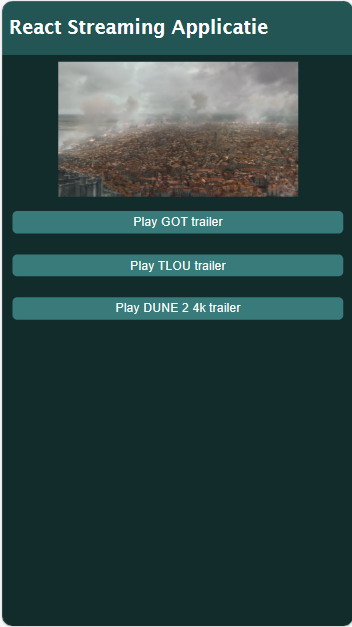
\includegraphics[width=0.7\linewidth]{img/ReactWebsiteIphone}
  \caption{React-website op een iPhone SE vanuit de browser.}
  \label{fig:React-website op een iPhone SE vanuit de browser}
\end{figure}

In het bestand 'App.js' wordt de hoofdstructuur van de website gedefinieerd. Allereerst wordt er binnen deze App-component een state bijgehouden voor de 'videoId' (ook wel de voorgedefinieerde constante die hoort bij een specifieke video uit de back-end) met behulp van de 'useState'-hook en wordt deze geïnitialiseerd met \verb|null|. Deze state houdt bij welke video momenteel wordt afgespeeld in de VideoPlayer-component.

Vervolgens is er een \verb|playVideo|-functie gedefinieerd binnenin de App-component. Deze functie wordt aangeroepen wanneer een van de afspeelknoppen wordt aangeklikt. De \verb|e.preventDefault()| -functie wordt aangeroepen om het eventuele standaardgedrag die ontstaat bij het klikken op een knop te voorkomen. Het zou bijvoorbeeld kunnen voorkomen dat de pagina opnieuw wordt geladen. Daarna wordt via de \verb|setVideoId|-functie de 'videoId'-state bijgewerkt naar de nieuwe waarde die overeenkomt met de gekozen video.

Als laatste retourneert dit component nog de JSX, of ook wel de daadwerkelijke interface van de website. Deze bestaat uit pure HTML in combinatie met de Header-, VideoPlayer- en de Button-componenten. Indien een button wordt aangeklikt, zal de \verb|playVideo|-functie aangeroepen worden en dus bijgevolg de 'videoId'-state worden bijgewerkt. Deze ID wordt op zijn beurt dan weer doorgegeven aan de VideoPlayer-component als parameter. Deze code van de App-component luidt als volgt:


\begin{LVerbatim}[language=JavaScript]
function App() {
  const [videoId, setVideoId] = useState(null);

  function playVideo(e, videoId) {
    e.preventDefault();
    setVideoId(videoId);
  };

  return (
    <div className="App">
      <Header/>
      <div className='content'>
        <div className='player'>
          {videoId && <VideoPlayer videoId={videoId}></VideoPlayer>} <br />
        </div>
        <div className='vidSelect'>
          <button onClick={(e) => playVideo(e, 'got')}>
            Play GOT trailer
          </button>
          <button onClick={(e) => playVideo(e, 'tlou')}>
            Play TLOU trailer
          </button>
          <button onClick={(e) => playVideo(e, 'dune')}>
            Play DUNE 2 4k trailer
          </button>
        </div>
      </div>
    </div>
  );
}
\end{LVerbatim}

De volgende en ook wel belangrijkste component in dit POC, is de VideoPlayer-component. Deze is verantwoordelijk voor het effectief afspelen van de geselecteerde video. Deze ontvang ten eerste een 'videoId' als parameter. Wanneer de 'videoId' zou veranderen in de App-component, zoals bij het aanklikken van een van bovenstaande knoppen, zal dit component volledig opnieuw renderen.

De VideoPlayer maakt daarnaast eerst en vooral gebruik van de 'useRef'-hook om een referentie te verkrijgen naar het <video>-element. Dit is nodig om toegang te verkrijgen tot de video zelf en om bepaalde eigenschappen te kunnen wijzigen. Dit wordt gedaan in de 'useEffect'-hook van de code. Het nut van deze hook is dat deze wordt aangeroepen na de eerste render van de component en na elke volgende update. Dit laat toe om bepaalde side-effects op te lossen. De rol van deze hook heeft vooral te maken met het re-renderen van de VideoPlayer indien de 'videoId' verandert. In dit geval zal de video gepauzeerd worden, de huidige source naar de video verwijderd worden en de video met de nieuwe source correct laden en afspelen. Zonder deze useEffect-hook zou indien een nieuwe video geselecteerd is, deze niet kunnen ingeladen worden en nog steeds een referentie hebben naar de oude source.

Tot slot retourneert dit component een <video>-element waarin de video wordt afgespeeld. De grootte van het video-element wordt dynamisch ingesteld op basis van de 'vidWidth' en 'vidHeight'-states uit het component. De source van de video wordt dynamisch toegekend aan de hand van een url naar de back-end API endpoint met de 'videoId' als parameter.

De code van de VideoPlayer ziet er als volgt uit. Om de leesbaarheid te verhogen tot enkel de belangrijkste aspecten uit de code, zijn enkele lijntjes code weggelaten die betrekking hebben tot de grootte van het venster van de video zelf. Deze hebben echter geen invloed op de prestaties van de website en/of applicatie zelf en behoren ook niet tot de scope van dit onderzoek. Let hierbij op dat de url naar de back-end deels is vervangen door de letter 'X' om privacyredenen. Dit kan vervangen worden door 'localhost', maar bleek de enige oplossing voor de Ionic-applicatie om lokaal de back-end te bereiken.

\begin{LVerbatim}[language=JavaScript, caption=Express API-endpoint voor het streamen van videobestanden]
const VideoPlayer = ({videoId}) => {
  const videoRef = useRef(null);

  useEffect(() => {
    if (videoRef.current) {
      videoRef.current.pause();
      videoRef.current.removeAttribute('src');
      videoRef.current.load();
    }
  });

  return (
    <video ref={videoRef} width={vidWidth} height={vidHeight} controls>
      <source src={`http://192.168.X.XXX:3000/videos/\${videoId}`}
        type="video/mkv"></source>
      Your browser does not support the video tag.
    </video>
  );
}
\end{LVerbatim}


\subsection{Ionic applicatie}
\label{sec:ionic-applicatie}

Nu de React-website is opgezet, kan er overgegaan worden tot het ontwikkelen en/of omzetten naar de mobiele applicaties. Uit hoofdstuk \ref{sec:ionic} bleek dat er eigenlijk geen verdere aanpassingen hoeven te gebeuren aan de bestaande React-website om deze te kunnen omzetten naar een Ionic-applicatie. Ter verduidelijking werd er voor deze Ionic-applicatie gebruik gemaakt van het React-framework, alhoewel er hiervoor ook de keuze is om een andere, door Ionic ondertsteund framework, te gebruiken. Dit heeft als troef dat de originele website-codebase letterlijk kan worden hergebruikt voor de mobiele applicatie.

Deze conversie gebeurt aan de hand van de Capacitor-plugin v6.0.0. De Ionic-applicatie zelf is dan weer gebouwd met versie 7.2.0 van Ionic. De combinatie van deze twee plugins maakt het mogelijk om de React-website te converteren naar een native-applicatie voor Android. Dit wordt bereikt door het aanmaken van twee bestanden: \verb|ionic.config.json| en \verb|capacitor.config.json|. Dit eerste bestand bevat the instellingen voor de Ionic-applicatie, zoals de naam en het feit dat deze applicatie steunt op React. Dit ziet er als volgt uit:

\begin{LVerbatim}[language=JavaScript]
{
  "name": "IonicStreaming",
  "integrations": {
    "capacitor": {}
  },
  "type": "react"
}
\end{LVerbatim}

Het tweede bestand bevat dan weer configuraties voor de Capacitor-plugin. De inhoud hiervan ziet er zo uit:

\begin{LVerbatim}[language=JavaScript]
{
  "appId": "io.ionic.IonicStreaming",
  "appName": "IonicStreaming",
  "bundledWebRuntime": false,
  "npmClient": "npm",
  "webDir": "build",
  "cordova": {}
}
\end{LVerbatim}

Na het aanmaken van deze bestanden is het nodig om de huidige website eerst te builden. Dit komt omdat Capacitor geen ingebouwde build-tool heeft en gebruik maakt van de bestaande build van de React-website. Door het commando \verb|npm run build| uit te voeren, worden de nodige bestanden gegenereerd in de 'build'-map in de root folder van het project. Er rest nog een laatste stap en dat is het effectief converteren naar een Android-applicatie. Het commando \verb|ionic capacitor add android| zorgt hiervoor.

Nadat deze applicatie is geconverteerd, hebben we onze definitieve Ionic-applicatie. Dit zonder enig lijntje van de originele codebase aan te passen. De applicatie kan nu worden gebuild via Gradle en geïnstalleerd op een Android-toestel. Er is echter nog een klein probleem bij deze build en dit heeft allemaal te maken met de lokaal draaiende back-end. Omdat deze via de localhost bereikbaar is, moet het commando \verb|ionic cap run android| \verb|-l --external| worden uitgevoerd. Dit is enkel en alleen nodig in dit specifieke geval: indien de API-endpoint bereikbaar is via een externe HTTPS-verbinding, is dit niet nodig. Wat dit commando doet is de vorige stappen zelf opnieuw uitvoeren, maar de applicatie bovendien ook lokaal draaien op localhost. Dit kan best vergeleken worden met de Ionic-applicatie te draaien op een bepaalde poort, zoals de originele React-website zou doen. Door deze tussenstap te nemen, kan de app opgestart worden met Android Studio en toch de back-end via de lokale pc bereiken.

Een screenshot van de applicatie staat op de volgende pagina.

\begin{figure}
  \centering
  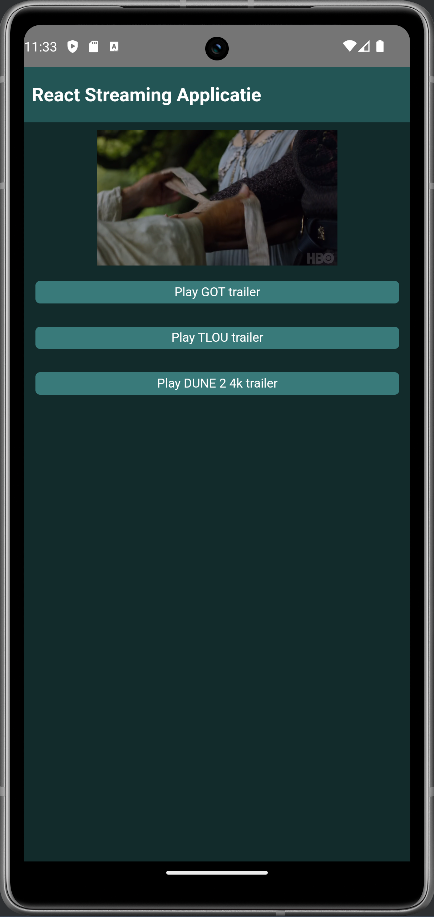
\includegraphics[width=0.7\linewidth]{img/ReactIonicPhone}
  \caption{Ionic-applicatie op een Google Pixel 7a}
  \label{fig:Ionic-applicatie op een Google Pixel 7a}
\end{figure}

Door deze bovenstaande stappen te volgen was het dus mogelijk om zonder enige aanpassingen, de React-website te deployen als een native Android-applicatie. Dit toont aan dat de combinatie van React, Ionic en Capacitor een krachtige toolset is om webapplicaties om te zetten naar mobiele applicaties. Wat natuurlijk weer een voordeel is voor ontwikkelaars om niet een volledig nieuwe applicatie te moeten herimplementeren.

\subsection{React Native applicatie}
\label{sec:react-native-applicatie}

Het laatste deel van de opzetting voor de testscenario's is de React Native-conversie. In tegenstelling tot een Ionic-applicatie, steunt deze niet op de typische webtechnologie van HTML, maar maakt gebruikt van eigen custom componenten. Dit wil betekenen dat de React-website niet zomaar kan worden omgezet naar een React Native-applicatie zoals bij Ionic. Desondanks is deze omzetting wel mogelijk omdat React Native voor de meeste HTML-elementen een equivalent heeft. Dit laat toe om de meeste code toch op een relatief eenvoudige manier te kunnen hergebruiken, mits enkele aanpassingen die hier worden besproken.

\begin{LVerbatim}[language=JavaScript, caption=Express API-endpoint voor het streamen van videobestanden]
const App = () => {
  const [videoId, setVideoId] = useState(null);

  function playVideo(e, videoId) {
    e.preventDefault();
    setVideoId(videoId);
  };

  return (
    <View style={styles.app}>
      <Header />
      <View style={styles.content}>
          <VideoPlayer videoId={videoId}></VideoPlayer>
          <View style={styles.vidSelect}>
            <Button
              onPress={(e) => playVideo(e, 'got')}
              title='Play GOT trailer'
              color={'rgb(57, 122, 122)'}>
            </Button>
            <Button
              onPress={(e) => playVideo(e, 'tlou')}
              title='Play TLOU trailer'
              color={'rgb(57, 122, 122)'}>
            </Button>
            <Button
              onPress={(e) => playVideo(e, 'dune')}
              title='Play DUNE 2 4k trailer'
              color={'rgb(57, 122, 122)'}>
            </Button>
        </View>
      </View>
    </View>
  );
};
\end{LVerbatim}

Bovenstaande code toont de App-component van de React Native-applicatie. Deze is zeer gelijkaardig aan de App-component van de originele React-website. Het grootste verschil is dat de HTML-elementen vervangen zijn door React Native-componenten. Zo wordt de <div>-tag vervangen door de <View>-tag en de HTML-buttons door de <Button>-component. De styling werd ook identiek overgezet op basis van de React-website, maar heeft eigenlijk geen invloed op de werking van de applicatie zelf. Als er vervolgens gekeken wordt naar de VideoPlayer-component, is deze ook gelijkaardig opgebouwd als de React-website. Maar voor dit component bleek er toch één groot probleem: React Native biedt geen standaard video-component aan. Dit betekent dus dat er moet gesteund worden op een externe package. In dit geval werd er gekozen voor de 'react-native-video'-package. Deze light-weight package biedt een video-component aan die zeer gelijkaardig is aan de <video>-tag in HTML.

Er wordt daarnaast opnieuw gebruikt gemaakt van de 'useRef'-hook om een referentie te verkrijgen naar het video-element. De useEffect-hook bij Ionic wordt echter niet gebruikt aangezien de React Native-video-component zelf al een ingebouwde manier heeft om de video te pauzeren en te hervatten, en de source van de video automatisch laat wijzigen wanneer de 'videoId' verandert. Deze useEffect-hook is dus overbodig in dit geval.

Voor de connectie met localhost is er geen extra configuratie nodig zoals bij de Ionic-applicatie. Slechts de url zoals in de onderstaande code bleek voldoende voor de connectie:

\begin{figure}
  \centering
  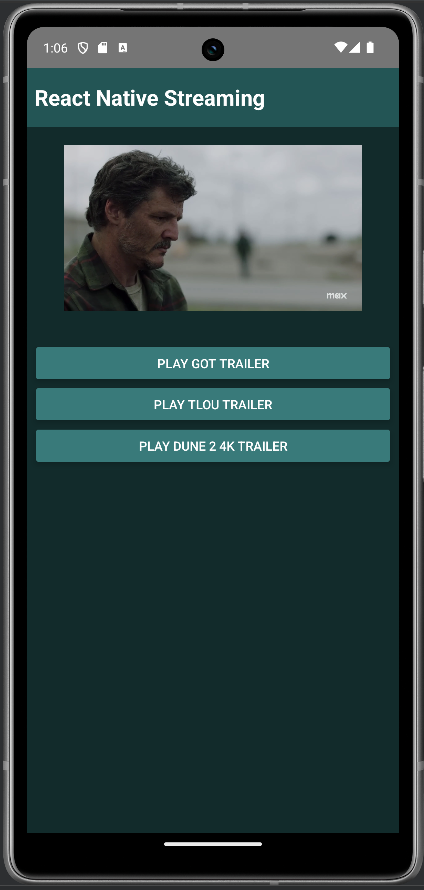
\includegraphics[width=0.7\linewidth]{img/ReactNativePhone}
  \caption{React Native-applicatie op een Google Pixel 7a}
  \label{fig:React Native-applicatie op een Google Pixel 7a}
\end{figure}

\begin{LVerbatim}[language=JavaScript]
const VideoPlayer = ({videoId}) => {
  const videoRef = useRef(null);

  return (
    <View style={styles.videoView}>
      <Video 
        source={{uri: `http://10.0.2.2:3000/videos/${videoId}`}} 
        ref={(ref) => {
          videoRef.current = ref;
        }}         
        style={styles.backgroundVideo}
      />
    </View>
  )
}
\end{LVerbatim}

Nu de code is geschreven is het enkel nog een kwestie van de applicatie te builden en te deployen naar een Android-toestel. Hiervoor werd er in de package.json volgende script toegevoegd:

\begin{LVerbatim}[language=JavaScript, caption=Express API-endpoint voor het streamen van videobestanden]
"build": "react-native bundle --platform android
    --dev false --entry-file index.js
    --bundle-output android/app/src/main/assets/index.android.bundle
    --assets-dest android/app/src/main/res"
\end{LVerbatim}

%++ metro v0.80.8

Dit script zorgt ervoor dat de code wordt gebundeld en dat de nodige bestanden worden gegenereerd in de 'android/app/src/main/assets'-map van de root-folder. Vervolgens kan deze build worden geopend in Android Studio en kan de applicatie via Gradle worden gebuild en geïnstalleerd op een Android-toestel. De afbeelding op de volgende pagina toont de React Native-applicatie op een Google Pixel 7a. Enkele verschillen zijn misschien merkbaar in de styling tussen de verschillende versies, maar dit heeft opnieuw geen invloed op de performantie van de applicatie en eerder te maken met de beperkte styling die React Native aan zijn componenten geeft. Bovendien werd de styling zo goed als helemaal overgenomen van de originele React-website (en dus ook Ionic-applicatie), dus deze kleine verschillen zijn als het ware verwaarloosbaar.

\section{Testscenario's}
\label{sec:testscenario}

Met de ontwikkeling van zowel de Ionic- als de React Native-applicaties nu voltooid, kan er overgegaan worden naar de testfase van dit Proof-of-Concept. In deze fase zal er onder andere gekeken worden naar de algemene opstarttijden, gebruikerservaring bij de interactie met de applicatie, alsook metingen worden gedaan met betrekking tot het CPU- en geheugenverbruik.


\subsection{Cold startup-tijd}
\label{subsec:cold-startup-tijd}

De term cold startup-tijd verwijst naar de tijd die nodig is voor een applicatie om op te starten vanaf het begin. Dit in een situatie waarbij de applicatie nog niet is geopend (zoals bij het opstarten van het toestel) of bij het volledig afsluiten van de app. Deze meting werd uitgevoerd door de applicatie eerst telkens volledig af te sluiten door een 'force stop' uit te voeren op de emulator en vervolgens de applicatie opnieuw te openen. Aan de hand van de logs en de Profiler van Android Studio kon de tijd gemeten worden vanaf het aanklikken van het icoon, tot wanneer de componenten volledig zijn ingeladen op het scherm. Er valt hierbij op te merken dat het videocomponent nog niet wordt ingeladen vanwege het feit dat er geen video is geselecteerd. Dit wordt in een latere fase onderzocht.

Dit waren de resultaten na zes metingen:

\begin{table}[htbp]
  \centering
  \begin{tabular}{|c|c|c|}
    \hline
    \textbf{Testscenario} & \textbf{Ionic} & \textbf{React Native} \\
    \hline
    1 & 2s 961ms & 6s 539ms \\
    \hline
    2 & 3s 114ms & 6s 876ms \\
    \hline
    3 & 3s 191ms & 6s 967ms \\
    \hline
    4 & 2s 987ms & 6s 477ms \\
    \hline
    5 & 3s 73ms & 6s 826ms \\
    \hline
    6 & 3s 118ms & 6s 895ms \\
    \hline
    \textbf{Gemiddelde} & \textbf{3s 74ms} & \textbf{6s 763ms} \\
    \hline
  \end{tabular}
  \caption{Cold startup tijd voor Ionic en React Native applicaties}
  \label{tab:cold_startup}
\end{table}

Hieruit blijkt dat de cold startup-tijd voor de React Native applicatie een heel stuk langer is dan die van de Ionic-applicatie. De gemiddelde tijd voor de React Native-applicatie bedraagt gemiddeld 6 seconden, terwijl deze voor de Ionic-applicatie slechts 3 seconden bedraagt. Dit is meer dan het dubbel van de tijd die nodig is voor de Ionic-applicatie. Dit kan een belangrijke factor zijn voor de gebruikerservaring van een applicatie. Een verdere verklaring en interpretatie van deze resultaten wordt, zoals eerder vermeld, gegeven in het volgende hoofdstuk.

\subsection{Warm startup-tijd}
\label{subsec:warm-startup-tijd}

Warm startup-tijd verwijst naar de tijd die nodig is voor een applicatie om opnieuw te starten nadat deze al een keer is gestart geweest en enige tijd inactief is geweest. Dit is te vergelijken met een gebruiker die de applicatie opnieuw opent nadat deze al een keer is geopend en vervolgens is geminimaliseerd, om bijvoorbeeld te surfen op het internet. Dit omvat dus het opnieuw inladen van de applicatie, waarbij de resources voor een deel of volledig nog in het geheugen zijn opgeslagen. Deze meting werd uitgevoerd door de applicatie te openen, te minimaliseren, Google Chrome te openen en weer te minimaliseren, en vervolgens de Ionic- en React Native-app weer te openen. De tijd werd gemeten vanaf het aanklikken van het icoon tot wanneer de componenten volledig zijn ingeladen op het scherm op basis van de logs en de Profiler van Android Studio.

\begin{table}[htbp]
  \centering
  \begin{tabular}{|c|c|c|}
  \hline
  \textbf{Testscenario} & \textbf{Ionic} & \textbf{React Native} \\
  \hline
  1 & 239ms & 239ms \\
  \hline
  2 & 328ms & 237ms \\
  \hline
  3 & 301ms & 195ms \\
  \hline
  4 & 283ms & 232ms \\
  \hline
  5 & 241ms & 217ms \\
  \hline
  6 & 319ms & 200ms \\
  \hline
  \textbf{Gemiddelde} & \textbf{285ms} & \textbf{220ms} \\
  \hline
  \end{tabular}
  \caption{Warm startup-tijd voor Ionic en React Native applicaties}
  \label{tab:warm_startup}
\end{table}

In vergelijking met de cold startup-tijd zijn de warme opstarttijden aanzienlijk korter, wat aangeeft dat het opnieuw starten minder tijd kost. Over het algemeen laten de metingen zien dat zowel Ionic als React Native relatief snelle warme opstarttijden hebben, waarbij React Native over het algemeen iets sneller lijkt te zijn dan Ionic, alhoewel dit verschil slechts over enkele milliseconden gaat.


\subsection{Interactie}
\label{subsec:interactie}

De interactie met de applicaties werd als vrij responsief ervaren. Het was mogelijk om vrij snel te schakelen tussen de verschillende video's door op de knoppen te klikken. Vanaf een knop werd aangeklikt, reageerde de interface onmiddellijk door de videospeler te renderen en binnen een tijdspanne van 2-3 seconden de video af te spelen. Ondanks dat er een pauze was tussen het klikken op de knop en het effectief inladen van de video, was deze pauze niet storend en werd de video snel en vloeiend afgespeeld. Bij het meten werd er deze keer opnieuw gekeken naar de Android Profiler en de logs van Android Studio om de reactietijden te meten. De resultaten van deze metingen zijn te vinden in de volgende tabel.

%erbij vermelden dat emulator stottert


\begin{table}[htbp]
  \centering
  \begin{tabular}{|c|c|c|}
  \hline
  \textbf{Testscenario} & \textbf{Ionic} & \textbf{React Native} \\
  \hline
  1 & 2s 807ms & 3s 56ms \\
  \hline
  2 & 2s 159ms & 2s 218ms \\
  \hline
  3 & 2s 123ms & 3s 177ms \\
  \hline
  4 & 2s 412ms & 2s 979ms \\
  \hline
  5 & 2s 788ms & 2s 762ms \\
  \hline
  6 & 2s 437ms & 2s 731ms \\
  \hline
  \textbf{Gemiddelde} & \textbf{2s 454ms} & \textbf{2s 820ms} \\
  \hline
  \end{tabular}
  \caption{Tijd voor het inladen van de video na het klikken op een knop voor Ionic en React Native applicaties}
  \label{tab:warm_startup}
\end{table}



Deze metingen laten zien dat React Native over het algemeen iets langzamer reageert dan bij Ionic met een verschil van bijna een halve seconde.
+ Nog wat uitgebreidere conclusie schrijven
    

\subsection{Video afspeelprestaties}
\label{subsec:video-afspeelprestaties}

Bij het afspelen van video's op zowel React als Ionic, werd over het algemeen een hoge afspeelkwaliteit ervaren. De video's werd telkens in hoge kwaliteit met een goed geluid afgespeeld. Echter werden er momenten waargenomen waarbij er enige haperingen optraden, vooral bij het afspelen van video's met de hogere resolutie van 4k. Hierdoor begon ook de geluidssynchronisatie wat te haperen en leek alsof beide applicaties wel wat moeite bleken te hebben.

Echter op basis van onderstaande metingen, blijkt dat de haperingen eerder te wijten zijn aan de emulator dan aan de applicaties zelf. Dit wordt ondersteund door observaties van het CPU-gebruik die op geen enkel moment werden overbelast. Daarnaast hapert de emulator zelf ook bij het algemeen gebruik, zoals bij het scrollen tussen de geïnstalleerde applicaties, met andere woorden bij laag intensief gebruik. Deze overhead wordt in het hoofdstuk verder geïnterpreteerd op basis van de resultaten uit de metingen.


\subsection{CPU-gebruik}
\label{subsec:cpu-gebruik}

Het CPU-gebruik werd telkens al volgt gemeten. Allereerst werd de applicatie de eerste keer opgestart nadat deze volledig was afgesloten. Vervolgens werd er een meting gedaan zonder dat er een video werd afgespeeld. Hierna werden beide 1080p video's getest en als laatste de 4k video. De metingen werden gedaan aan de hand van de Android Profiler in Android Studio. Hierbij werd er gekeken naar de CPU-gebruikspieken en -dalen die optraden tijdens de verschillende activiteiten.

Voor Ionic vertoonde de applicatie bij het opstarten een piek van 41\% CPU-gebruik. Zonder het afspelen van video's bleef het CPU-gebruik hierna tussen 0-1\%. Bij het afspelen van een 1080p video varieerde het CPU-gebruik tussen 22-37\%, met enkele dalingen van 12\% en pieken tot 43\% van het totale CPU-gebruik. Bij het afspelen van een 4k video waren er iets hogere variaties tussen 32-52\%, met een drop van 32\% en een piek van 68\%.

Bij de observatie van het CPU-gebruik bij React Native tijdens dezelfde activiteiten, valt op dat er bij het starten van de applicatie een piek van 50\% CPU-gebruik optreedt. Dit is een gelijkaardige piek zoals bij Ionic. Zonder het afspelen van video's bleef het CPU-gebruik tussen de 1-2\% zitten. Wanneer een 1080p video werd afgespeeld, varieert het CPU-gebruik tussen 35-41\% bij het inladen van de video en varieerde vervolgens tussen de 38-70\%, met enkele dalingen tot 20\% en hoge pieken tot zelfs 90\%. Bij het afspelen van een 4k video varieerde dit ook vrij hard, met een dieptepunt van 26\% en een piek van 92\%, en een algemene variatie tussen 35-82\%. 

Over het algemeen tonen deze observaties aan dat het CPU-gebruik vrij hoog kan zijn bij het afspelen van video's, vooral bij hogere resoluties zoals 4k. Dit kan leiden tot een hoger energieverbruik en een snellere batterijafvoer, wat belangrijk is om in overweging te nemen bij het ontwikkelen van video-intensieve applicaties. Daarnaast bleek ook dat React Native telkens een hoger CPU-gebruik had dan Ionic. Een mogelijke verklaring wordt later besproken.

\subsection{Geheugengebruik}
\label{subsec:geheugengebruik}

Het volgende aspect dat nader werd onderzocht, was het geheugengebruik. Deze metingen werden op het zelfde moment gedaan als de CPU-metingen. Hierbij werd vastgesteld dat zonder het inladen van video's, het geheugengebruik voor zowel React als Ionic relatief laag en stabiel bleef. Bij React Native bleek dit iets lager met een variatie tussen 110,2MB en 114,8MB, terwijl dit voor Ionic tussen 113,9MB en 116,8MB lag.

Wanneer een 1080p video werd afgespeeld, bleek het geheugengebruik voor React Native langzaamaan te stijgen tot 135,4MB om uiteindelijk af te vlakken bij 153,1MB. Voor het streamen van een 4k video steeg het geheugengebruik van 110,2MB tot 156,5MB en vlakte vervolgens ook weer af.

Het geheugengebruik bij Ionic kon wat variëren, maar dit gebeurde telkens in beperkte mate. Bij het afspelen van een 1080p video varieerde het geheugengebruik tussen 119,7MB en 128,2MB, met een plots dieptepunt van 113MB. Bij het afspelen van een 4k video bleek het geheugengebruik quasi hetzelfde met een enkel dieptepunt van 114MB.

Over het algemeen laten deze bevindingen zien dat zowel React als Ionic redelijk stabiel zijn omtrent geheugengebruik, met slechts lichte variaties afhankelijk van de resolutie van de video. Toch scoort Ionic op dit vlak opnieuw beter dan React Native.


\subsection{Groottes van de applicaties}
\label{subsec:groottes-van-de-applicaties}

(nog uit te schrijven)
%Wanneer we kijken naar de omvang van de APK-bestanden voor React en Ionic, zien we een aanzienlijk verschil. De APK-bestandsgrootte voor React bedraagt 155 MB, terwijl die voor Ionic slechts 3,76 MB is. Dit enorme verschil in bestandsgrootte kan verschillende oorzaken hebben, waaronder de complexiteit van de frameworks, de gebruikte bibliotheken en de manier waarop de applicaties worden gebouwd. Over het algemeen suggereert dit dat Ionic mogelijk lichtere en meer efficiënte APK-bestanden produceert in vergelijking met React, wat belangrijk kan zijn voor gebruikers met beperkte opslagruimte op hun apparaten of voor situaties waarin snelle download- en installatietijden van de applicatie van belang zijn.

React Native:
  - 155 MB .apk size

Ionic: 
  - 3.76 MB .apk size

(zeer opvallende situatie maar heeft waarschijnlijk te maken met het feit dat React Native de componenten in de app zelf moet inladen, terwijl Ionic gebruik maakt van de webview-engine van het toestel)